\section{Benchmarking Synthetic Tabular Data Generation Algorithms}
\label{sec:exp}

\subsection{Experimental Setups}
\textbf{Datasets}. We select six real-world tabular datasets consisting of both numerical and categorical attributes: Adult, Default, Shoppers, Magic, Faults, Beijing, and News. Table~\ref{tbl:exp-dataset} provides the overall statistics of these datasets, and the detailed descriptions can be found in Appendix~\ref{appendix:dataset}.

\textbf{Baselines}.
We compare the proposed \modelname with seven existing synthetic tabular data generation methods. The first two are classical GAN and VAE models: CTGAN~\citep{ctgan} and TVAE~\citep{ctgan}. Additionally, we evaluate five SOTA methods introduced recently: GOGGLE~\citep{goggle}, a VAE-based method; GReaT~\citep{great}, a language model variant; and three diffusion-based methods: STaSy~\citep{stasy}, TabDDPM~\citep{tabddpm}, and CoDi~\citep{codi}. Notably, these approaches were nearly simultaneously introduced, limiting opportunities for extensive comparison. For reference, we also compare with the representative interpolation-based method SMOTE~\citep{smote}. Our paper fills this gap by providing the first comprehensive evaluation of their performance in a standardized setting. 

\textbf{Evaluation Methods}. We evaluate the quality of the synthetic data from three aspects: 1) \textbf{Low-order statistics} -- \emph{column-wise density estimation} and \emph{pair-wise column correlation}, estimating the density of every single column and the correlation between every column pair (Section~\ref{sec:exp-low-order}). We also perform Classifier Two Sample Test (C2ST) to evaluate if the synthetic data can be detected from the real data via a machine learning model (Appendix~\ref{appendix:detection}); 2) \textbf{High-order metrics} -- \emph{$\alpha$-precision} and \emph{$\beta$-recall} scores~\citep{faithful} that measure the overall fidelity and diversity of synthetic data (the results are deferred to Appendix~\ref{appendix:quality}); 3) \textbf{Privacy Protection}: we also evaluate if the synthetic data is randomly sampled according to the distribution density rather than copied from the training data via Distance to Closest Records (DCR) in Appendix~\ref{appendix:dcr}; 4) Performance on \textbf{downstream tasks} -- \emph{machine learning efficiency} (MLE) and \emph{missing value imputation}. MLE is to compare the testing accuracy on real data when trained on synthetically generated tabular datasets. The performance on {privacy protection} is measured by MLE tasks that have been widely adopted in previous literature (Section~\ref{sec:exp-downstream}). We also extend \modelname for the missing value imputation task, which aims to fill in missing features/labels given partial column values (Appendix~\ref{appendix:imputation}). The reported results are averaged over $20$ randomly sampled synthetic data. The implementation details are in Appendix~\ref{appendix:experiments}.

\subsection{Estimating Low-order Statistics of Data Density}\label{sec:exp-low-order}

\textbf{Metrics}.  We employ the Kolmogorov-Sirnov Test (KST) for numerical columns and the Total Variation Distance (TVD) for categorical columns to quantify column-wise density estimation. For pair-wise column correlation, we use Pearson correlation for numerical columns and contingency similarity for categorical columns. The performance is measured by the difference between the correlations computed from real data and synthetic data. For the correlation between numerical and categorical columns, we first group numerical values into categorical ones via bucketing, then calculate the corresponding contingency similarity. Further details on these metrics are in Appendix~\ref{appendix:metric}. 

\begin{table}[t!] 
    \centering
    \caption{Error rate (\%) of \textbf{column-wise density estimation}. {\redbf{Bold Face}} represents the best score on each dataset. Lower values indicate more accurate estimation (superior results). \modelname outperforms the best generative baseline model by $86.0\%$ on average.} 
    \label{tbl:exp-shape}
    \small
    \begin{threeparttable}
    {
    \scalebox{0.92}
    {
	\begin{tabular}{lcccccc|cccc}
            \toprule[0.8pt]
            \textbf{Method} & \textbf{Adult} & \textbf{Default} & \textbf{Shoppers} & \textbf{Magic}  & \textbf{Beijing} &  \textbf{News} & \textbf{Average}  \\
            \midrule 
             SMOTE & $1.60${\tiny$\pm 0.23$} & $1.48${\tiny$\pm0.15$} & $2.68${\tiny$\pm0.19$} & $0.91${\tiny$\pm0.05$}  &$1.85${\tiny$\pm0.21$} &   $5.31${\tiny$\pm 0.46$} &  $2.30$ & \\
            \midrule
            CTGAN    & $16.84${\tiny$\pm$ $0.03$} & $16.83${\tiny$\pm$$0.04$} & $21.15${\tiny$\pm0.10$} & $9.81${\tiny$\pm0.08$}  &$21.39${\tiny$\pm0.05$} &   $16.09${\tiny$\pm 0
            .02$} & $17.02$  \\
            TVAE     & $14.22${\tiny$\pm0.08$} & $10.17${\tiny$\pm$$0.05$} & $24.51${\tiny$\pm0.06$} & $8.25${\tiny$\pm0.06$}  &  $19.16${\tiny$\pm0.06$}  &  $16.62${\tiny$\pm0.03$} &  $15.49$   \\
            GOGGLE$^{1}$   & $16.97$ & $17.02$ & $22.33$ & $1.90$  & $16.93 $ &   $25.32$  &  $16.74$ \\
            GReaT$^{2}$     & $12.12${\tiny$\pm$$0.04$} & $19.94${\tiny$\pm$$0.06$}  & $14.51${\tiny$\pm0.12$}  &  $16.16${\tiny$\pm0.09$}   & $8.25${\tiny$\pm0.12$}  &  OOM &  $14.20$ \\
            STaSy    & $11.29${\tiny$\pm0.06$} & $5.77${\tiny$\pm0.06$} & $9.37${\tiny$\pm0.09$} & $6.29${\tiny$\pm0.13$}   & $6.71${\tiny$\pm0.03$}  &  $6.89${\tiny$\pm0.03$} &  $7.72$ \\
            CoDi  & $21.38${\tiny$\pm0.06$}  & $15.77${\tiny$\pm$ $0.07$}  & $31.84${\tiny$\pm0.05$}  & $11.56${\tiny$\pm0.26$}  & $16.94${\tiny$\pm0.02$} &    $32.27${\tiny$\pm0.04$} &  $21.63$  \\
            TabDDPM$^{3}$ & $1.75${\tiny$\pm0.03$}  & $1.57${\tiny$\pm$ $0.08$}  & $2.72${\tiny$\pm0.13$}  & $1.01${\tiny$\pm0.09$}   & $1.30${\tiny$\pm0.03$}  &  $78.75${\tiny$\pm0.01$} &  $14.52$ \\
            \midrule
            \modelname  & $\redbf{0.58}${\tiny$\redbf{\pm0.06}$} & $\redbf{0.85}${\tiny$\redbf{\pm0.04}$} & $\redbf{1.43}${\tiny$\redbf{\pm0.24}$} & $\redbf{0.88}${\tiny$\redbf{\pm0.09}$}  & $\redbf{1.12}${\tiny$\redbf{\pm0.05}$} & $\redbf{1.64}${\tiny$\redbf{\pm0.04}$}  &  $\redbf{1.08} $ \\
            Improv. &  $\redbf{66.9 \% \downarrow} $ & $ \redbf{45.9\% \downarrow} $ & $\redbf{47.4\% \downarrow}$ & $\redbf{12.9\% \downarrow} $  & $\redbf{13.8\% \downarrow }$  &  $\redbf{76.2\% \downarrow }$ &  $\redbf{86.0\% \downarrow }$ &  \\
		\bottomrule[1.0pt] 
		\end{tabular}
              }
              }
  		\begin{tablenotes}
            \item[1] GOGGLE fixes the random seed during sampling in the official codes, and we follow it for consistency.
            \item[2] GReaT cannot be applied on News because of the maximum length limit.
    	\item[3] TabDDPM fails to generate meaningful content on the News dataset.
        \end{tablenotes}
	\end{threeparttable}

\end{table}

\begin{table}[t!] 
    \centering
    \caption{Error rate (\%) of \textbf{pair-wise column} correlation score. {\redbf{Bold Face}} represents the best score on each dataset. \modelname outperforms the best baseline model by $67.6\%$ on average.} 
    \label{tbl:exp-trend}
    \small
% \begin{threeparttable}
    {
    \scalebox{0.93}
    {
	\begin{tabular}{lcccccc|ccc}
            \toprule[0.8pt]
            \textbf{Method} & \textbf{Adult} & \textbf{Default} & \textbf{Shoppers} & \textbf{Magic}  & \textbf{Beijing} & \textbf{News} & \textbf{Average}  \\
            \midrule 
             SMOTE & $3.28${\tiny$\pm0.29$} & $8.41${\tiny$\pm0.38$} & $3.56${\tiny$\pm0.22$} & $3.16${\tiny$\pm0.41$}  &$2.39${\tiny$\pm0.35$} &   $5.38${\tiny$\pm 0.76$} & $4.36$ & \\
            \midrule
            CTGAN    & $20.23${\tiny$\pm1.20$} & $26.95${\tiny$\pm0.93$} & $13.08${\tiny$\pm0.16$} & $7.00${\tiny$\pm0.19$} &  $22.95${\tiny$\pm0.08$}  &  $5.37${\tiny$\pm0.05$} & $15.93$     \\
            TVAE     & $14.15${\tiny$\pm0.88$} & $19.50${\tiny$\pm$$0.95$} & $18.67${\tiny$\pm0.38$} &  $5.82${\tiny$\pm0.49$}  &  $18.01${\tiny$\pm0.08$}  & $6.17${\tiny$\pm0.09$} & $13.72$   \\
            GOGGLE   & $45.29$ & $21.94$ & $23.90$ & $9.47$  & $45.94$  & $23.19$ & $28.28$   \\
            GReaT    & $17.59${\tiny$\pm0.22$} & $70.02${\tiny$\pm$$0.12$} & $45.16${\tiny$\pm0.18$} & $10.23${\tiny$\pm0.40$}  & $59.60${\tiny$\pm0.55$} & OOM   & $44.24$  \\
            STaSy    & $14.51${\tiny$\pm0.25$} & $5.96${\tiny$\pm$$0.26$}  & $8.49${\tiny$\pm0.15$} & $6.61${\tiny$\pm0.53$}  & $8.00${\tiny$\pm0.10$} & $3.07${\tiny$\pm0.04$} & $7.77$     \\
            CoDi  & $22.49${\tiny$\pm0.08$}  & $68.41${\tiny$\pm$$0.05$}  & $17.78${\tiny$\pm0.11$}  & $6.53${\tiny$\pm0.25$} & $7.07${\tiny$\pm0.15$} & $11.10${\tiny$\pm0.01$} & $22.23$   \\ 
            TabDDPM & $3.01${\tiny$\pm0.25$}  & $4.89${\tiny$\pm0.10$}  & $6.61${\tiny$\pm0.16$} & $1.70${\tiny$\pm0.22$} & $2.71${\tiny$\pm0.09$} & $13.16${\tiny$\pm0.11$} & $5.34$ \\
            \midrule
            \modelname  & $\redbf{1.54}${\tiny$\redbf{\pm0.27}$} & $\redbf{2.05}${\tiny$\redbf{\pm0.12}$} & $\redbf{2.07}${\tiny$\redbf{\pm0.21}$}  & $\redbf{1.06}${\tiny$\redbf{\pm0.31}$}   &  $\redbf{2.24}${\tiny$\redbf{\pm0.28}$}  & $\redbf{1.44}${\tiny$\redbf{\pm0.03}$} & $\redbf{1.73}$  \\
            Improve. &  $\redbf{48.8\% \downarrow} $ & $\redbf{58.1\% \downarrow} $ & $\redbf{68.7\% \downarrow}$  & $\redbf{37.6\% \downarrow} $  & $\redbf{17.3\% \downarrow} $  &  $\redbf{53.1\% \downarrow}$ & $\redbf{67.6\% \downarrow}$&  \\
		\bottomrule[1.0pt] 
		\end{tabular}
  }
  }
	% \end{threeparttable}
\end{table}

\paragraph{Column-wise distribution density estimation.} In Table~\ref{tbl:exp-shape}, we note that \modelname consistently outperforms baseline methods in the column-wise distribution density estimation task. On average, \modelname surpasses the most competitive baselines by $86.0\%$. While STaSy and TabDDPM perform well, STaSy is sub-optimal because it treats one-hot embeddings of categorical columns as continuous features. Additionally, TabDDPM exhibits unstable performance across datasets, failing to generate meaningful content on the News dataset despite a standard training process.

\paragraph{Pair-wise column correlations.} Table~\ref{tbl:exp-trend} displays the results of pair-wise column correlations. \modelname outperforms the best baselines by an average of $67.6\%$. Notably, the performance of GReaT is significantly poorer in this task than in the column-wise task. This indicates the limitations of autoregressive language models in density estimation, particularly in capturing the joint probability distributions between columns.

\subsection{Performance on Downstream Tasks}\label{sec:exp-downstream}
\paragraph{Machine Learning Efficiency.}
We then evaluate the quality of synthetic data by evaluating their performance in Machine Learning Efficiency tasks. Following established settings~\citep {tabddpm, stasy, codi}, we first split a real table into a real training and a real testing set. The generative models are learned on the real training set, from which a synthetic set of equivalent size is sampled. This synthetic data is then used to train a classification/regression model (XGBoost Classifier and XGBoost Regressor~\citep{xgboost}), which will be evaluated using the real testing set. The performance of MLE is measured by the AUC score for classification tasks and RMSE for regression tasks. The detailed settings of the MLE evaluations are in Appendix~\ref{appendix:mle}.

In Table~\ref{tbl:exp-mle}, we demonstrate that \modelname consistently outperforms all the baseline methods. The performance gap between methods is smaller compared to column-wise density and pair-wise column correlation estimation tasks (Tables~\ref{tbl:exp-shape} and~\ref{tbl:exp-trend}). This suggests that some columns may not significantly impact the classification/regression tasks, allowing methods with lower performance in previous tasks to show competitive results in MLE (e.g., GReaT on Default dataset). This underscores the need for a comprehensive evaluation approach beyond just MLE metrics. As shown above, we have incorporated low-order and high-order statistics for a more robust assessment.

\begin{table}[t!] 
    \centering
    \caption{AUC (classification task) and RMSE (regression task) scores of \textbf{Machine Learning Efficiency}. $\uparrow$ ($\downarrow$) indicates that the higher (lower) the score, the better the performance. \modelname consistently outperforms all others across all datasets.} 
    \label{tbl:exp-mle}
    \small
    \begin{threeparttable}
    {
    \scalebox{0.92}
    {
	\begin{tabular}{lcccccc|cc}
            \toprule[0.8pt]
            \multirow{2}{*}{Methods} & {\textbf{Adult}} &{\textbf{Default}} & \textbf{Shoppers} & {\textbf{Magic}} &   {\textbf{Beijing}} & {\textbf{News}}$^1$ & {\textbf{Average Gap}} \\
            \cmidrule{2-8} 
            & AUC $\uparrow$ & AUC $\uparrow$ &  AUC $\uparrow$ &  AUC $\uparrow$  & RMSE $\downarrow$ &  RMSE $\downarrow$ & $\%$ \\
            \midrule 
            Real & $.927${\tiny$\pm.000$} & $.770${\tiny$\pm.005$} & $.926${\tiny$\pm.001$}  & $.946${\tiny$\pm.001$}  & $.423${\tiny$\pm.003$} & $.842${\tiny$\pm.002$} & $0\%$  \\
            \midrule
            SMOTE & $.899${\tiny$\pm.007$} &$.741${\tiny$\pm.009$} & $.911${\tiny$\pm.012$} & $.934${\tiny$\pm.008$} & $.593${\tiny$\pm.011$} & $.897${\tiny$\pm.036$} & $9.39\%$  \\
            \midrule
            CTGAN & $.886${\tiny$\pm.002$} &$.696${\tiny$\pm.005$} & $.875${\tiny$\pm.009$} & $.855${\tiny$\pm.006$}    & $.902${\tiny$\pm.019$} & $.880${\tiny$\pm.016$} & $24.5\%$ \\
            TVAE  & $.878${\tiny$\pm.004$} &$.724 ${\tiny$\pm.005$} & $.871${\tiny$\pm.006$} & $.887${\tiny$\pm.003$} & $.770${\tiny$\pm.011$} & $1.01${\tiny$\pm.016$} & $20.9\%$  \\
            GOGGLE & $.778${\tiny$\pm.012$} & $.584${\tiny$\pm.005$} & $.658${\tiny$\pm.052$} & $.654${\tiny$\pm.024
            $}  & $1.09${\tiny$\pm.025$} & $.877${\tiny$\pm.002$} & $43.6\%$  \\
            GReaT & $.913${\tiny$\pm.003$} &$.755${\tiny$\pm.006$} & $.902${\tiny$\pm.005$} & $.888${\tiny$\pm.008$}  & $.653${\tiny$\pm.013$} & OOM  & $13.3\%$  \\
            STaSy  & $.906${\tiny$\pm.001$} & $.752${\tiny$\pm.006$} & $.914${\tiny$\pm.005$} & $.934${\tiny$\pm.003$}  & $.656${\tiny$\pm.014$} & $.871${\tiny$\pm.002$} & $10.9\%$  \\ 
            CoDi & $.871${\tiny$\pm.006$} & $.525${\tiny$\pm.006$} & $.865${\tiny$\pm.006$} & $.932${\tiny$\pm.003$}   & $.818${\tiny$\pm.021$} & $1.21${\tiny$\pm.005$} & $30.5\%$  \\
            TabDDPM$^2$ & $.907${\tiny$\pm.001$}  & $.758${\tiny$\pm.004$}& $.918${\tiny$\pm.005$} & $.935${\tiny$\pm.003$} & $.592${\tiny$\pm.011$}& $4.86${\tiny$\pm3.04$} & $9.14\%^1$ \\
            \midrule
            \modelname  & $\redbf{.915}${\tiny$\redbf{\pm.002}$} & $\redbf{.764}${\tiny$\redbf{\pm.004}$} & $\redbf{.920}${\tiny$\redbf{\pm.005}$} & $\redbf{.938}${\tiny$\redbf{\pm.002}$} &  $\redbf{.582}${\tiny$\redbf{\pm.008}$} & $\redbf{.861}${\tiny$\redbf{\pm.027}$} & $\redbf{7.23\%}$ 
            \\
		\bottomrule[1.0pt] 
		\end{tabular}
  }
  }
     \begin{tablenotes}
     \item[1] Following CoDi~\citep{codi}, the continuous targets are standardized to prevent large values.
    \item[2] TabDDPM collapses on News, leading to an extremely high error on this dataset. We exclude this dataset \\ when computing the average gap of TabDDPM.
        \end{tablenotes}
	\end{threeparttable}
\end{table}

\paragraph{Missing Value Imputation.} 
One advantage of the diffusion model is that a well-trained unconditional model can be directly used for data imputation (e.g., image inpainting~\citep{vp, repaint}) without additional training. This paper explores adapting \modelname for missing value imputation, a crucial task in real-world tabular data. Due to space limitation, the detailed algorithms for missing value imputation and the results are deferred to Appendix~\ref{appendix:imputation}.

\subsection{Ablation Studies}\label{sec:exp-ablation}
\paragraph{The effect of adaptive $\beta$-VAE.} We assess the effectiveness of scheduling the weighting coefficient $\beta$ in the VAE model. Figure~\ref{fig:beta} presents the trends of the reconstruction loss and the KL-divergence loss with the scheduled $\beta$ and constant $\beta$ values (from $10^{-1}$ to $10^{-5}$) across 4,000 training epochs. Notably, a large $\beta$  value leads to subpar reconstruction, while a small $\beta$ value results in a large divergence between the embedding distribution and the standard Gaussian, making the balance hard to achieve. In contrast, by dynamically scheduling $\beta$ during training  ($\beta_{\rm max} = 0.01, \beta_{\rm min} = 10^{-5}, \lambda = 0.7$), we not only prevent excessive KL divergence but also enhance quality. Table~\ref{tbl:beta} further evaluates the learned embeddings from various $\beta$ values of the VAE model via synthetic data quality (single-column density and pair-wise column correlation estimation tasks). This demonstrates the superior performance of our proposed scheduled $\beta$ approach to train the VAE model.
\begin{figure}[t]
\begin{minipage}[h]{0.65\linewidth}
    \vspace{0pt}
    \centering
    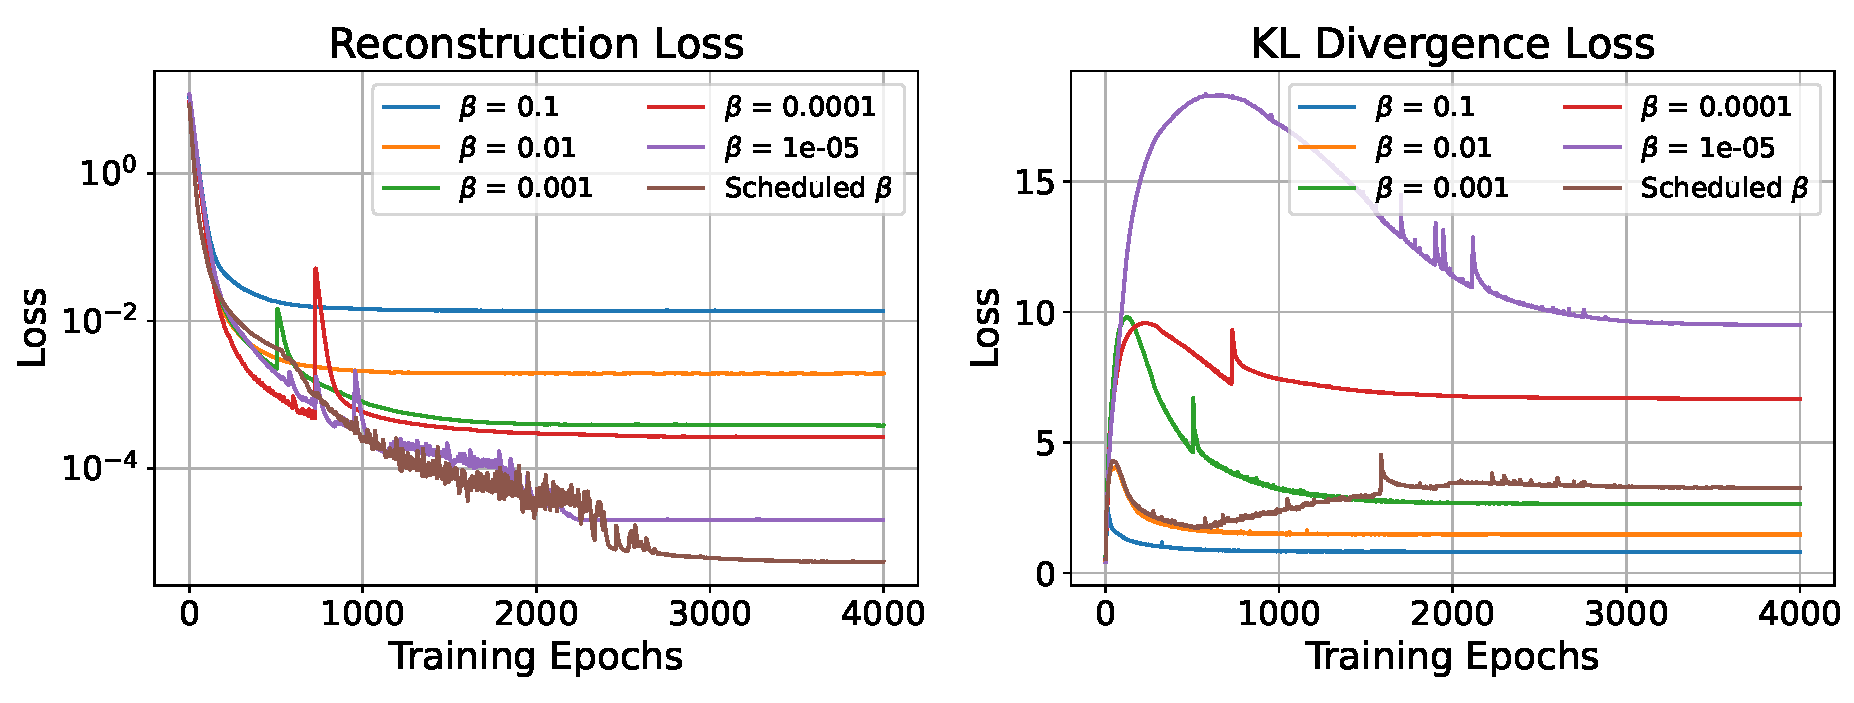
\includegraphics[width=1.0\textwidth,angle=0]{Fig/beta.pdf}
    \caption{The trends of the validation reconstruction (left) and KL-divergence (right) losses on the Adult dataset, with varying constant $\beta$, and our proposed scheduled $\beta$ ($\beta_{\rm max} = 0.01, \beta_{\rm min} = 10^{-5}, \lambda = 0.7$). The proposed scheduled $\beta$ obtains the lowest reconstruction loss with a fairly low KL-divergence loss.}
    \label{fig:beta}
\end{minipage}
\hspace{0.04\textwidth}
\begin{minipage}[h]{0.3\linewidth}
    \vspace{0pt}
    \centering
    \captionof{table}{The results of single-column density and pair-wise column correlation estimation with different $\beta$ values on the Adult dataset.}
    \label{tbl:beta}
    \small
    % \setlength{\tabcolsep}{0.8mm}
    % \begin{threeparttable}
    {
    \scalebox{0.9}{
	\begin{tabular}{ccccc}
            \toprule[1.0pt]
            $\beta$ & Single & Pair \\
            \midrule
            $10^{-1}$ & $1.24$ & $3.05$ \\
            $10^{-2}$ & $0.87$ & $2.79$ \\
            $10^{-3}$ & $0.72$ & $2.25$ \\
            $10^{-4}$ & $0.69$ & $2.01$ \\
            $10^{-5}$ & $41.96$ & $69.17$ \\
            Scheduled $\beta$& $\mathbf{0.58}$ &  $\mathbf{1.54}$ \\
		\bottomrule[1.0pt] 
		\end{tabular}
        }
        }
\end{minipage}
\end{figure}

\paragraph{The effect of linear noise levels.} We evaluate the effectiveness of using linear noise levels, $\sigma(t) = t$, in the diffusion process. As Section~\ref{sec:diffusion} outlines, linear noises lead to linear trajectories and faster sampling speed. Consequently, we compare \modelname and two other diffusion models (STaSy and TabDDPM) in terms of the single-column density and pair-wise column correlation estimation errors relative to the number of function evaluations (NFEs), i.e., denoising steps to generate the real data. As continuous-time diffusion models, the proposed \modelname and STaSy are flexible in choosing NFEs. For TabDDPM, we use the DDIM sampler~\citep{ddim} to adjust NFEs. Figure~\ref{fig:nfe} shows that \modelname not only significantly improves the sampling speed but also consistently yields better performance (with fewer than 20 NFEs for optimal results). In contrast, STaSy requires 50-200 NFEs, varying by datasets, and achieves sub-optimal performance. TabDDPM achieves competitive performance with 1,000 NFEs but significantly drops in performance when reducing NFEs.
\begin{figure}[t]
\begin{minipage}[h]{0.7\linewidth}
    \vspace{0pt}
    \centering
    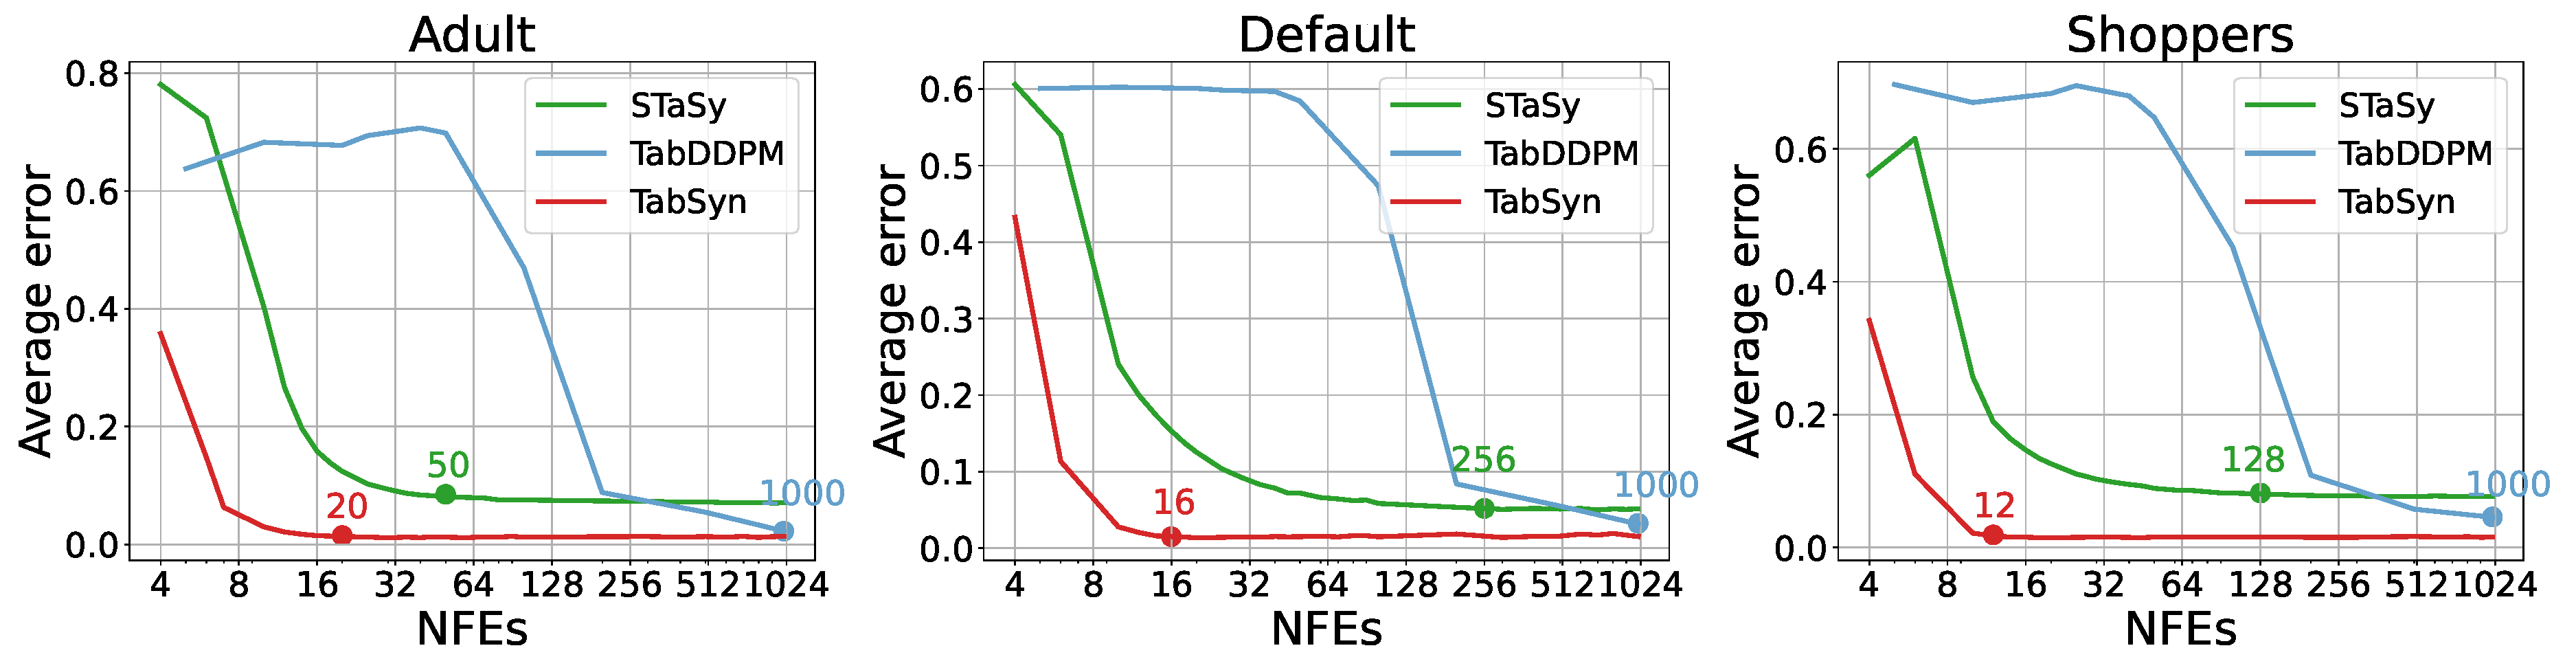
\includegraphics[width = 1.0\linewidth]{Fig/nfe.pdf}
    \caption{Quality of synthetic data as a function of NFEs on STaSy, TabDDPM, and \modelname. \modelname can generate synthetic data of the best quality with fewer NFEs (indicating faster sampling speed).}
    \label{fig:nfe}
\end{minipage}
\begin{minipage}[h]{0.28\linewidth}
    \vspace{0pt}
    \centering
    \captionof{table}{Performance of \modelname's variants on Adult dataset, on low-order statistics estimation tasks.}
    \label{tbl:ablation}
    \small
    % \setlength{\tabcolsep}{0.8mm}
    % \begin{threeparttable}
    {
    \scalebox{0.8}{
	\begin{tabular}{ccccc}
            \toprule[1.0pt]
            Variants & Single & Pair \\
            \midrule
            TabDDPM & $1.75$ & $3.01$ \\
            \midrule
            \modelname-OneHot & $5.59$ & $6.92$ \\
            \modelname-DDPM & $1.02$ & $2.15$ \\
            \midrule
            \modelname & $\mathbf{0.58}$ &  $\mathbf{1.54}$ \\
		\bottomrule[1.0pt] 
		\end{tabular}
        }
        }
\end{minipage}
\vspace{-12pt}
\end{figure}

\paragraph{Comparing different encoding/diffusion methods.}
We assess the effectiveness of learning the diffusion model in the latent space learned by VAE by creating two \modelname variants: 1) \modelname-OneHot: replacing VAE with one-hot encodings of categorical variables and 2) \modelname-DDPM: substituting the diffusion process in Equation~(\ref{eqn:forward}) with DDPM as used in TabDDPM. Results in Table~\ref{tbl:ablation} demonstrate: 1) One-hot encodings for categorical variables plus continuous diffusion models lead to the worst performance, indicating that it is not appropriate to treat categorical columns simply as continuous features; 2) \modelname-DDPM in the latent space outperforms TabDDPM in the data space, highlighting the benefit of learning high-quality latent embeddings for improved diffusion modeling; 3) \modelname surpasses \modelname-DDPM, indicating the advantage of employing tailored diffusion models in the continuous latent space for better data distribution learning.

\subsection{Visualization}
 In Figure~\ref{fig:case-single}, we compare column density across eight columns from four datasets (one numerical and one categorical per dataset). TabDDPM matches \modelname's accuracy on numerical columns but falls short on categorical ones. Figure~\ref{fig:case-pair} displays the divergence heatmap between estimated pair-wise column correlations and real correlations. \modelname gives the most accurate correlation estimation, while other methods exhibit suboptimal performance. These results justify that employing generative modeling in latent space enhances the learning of categorical features and joint column distributions.
\begin{figure}[t]
  \centering
  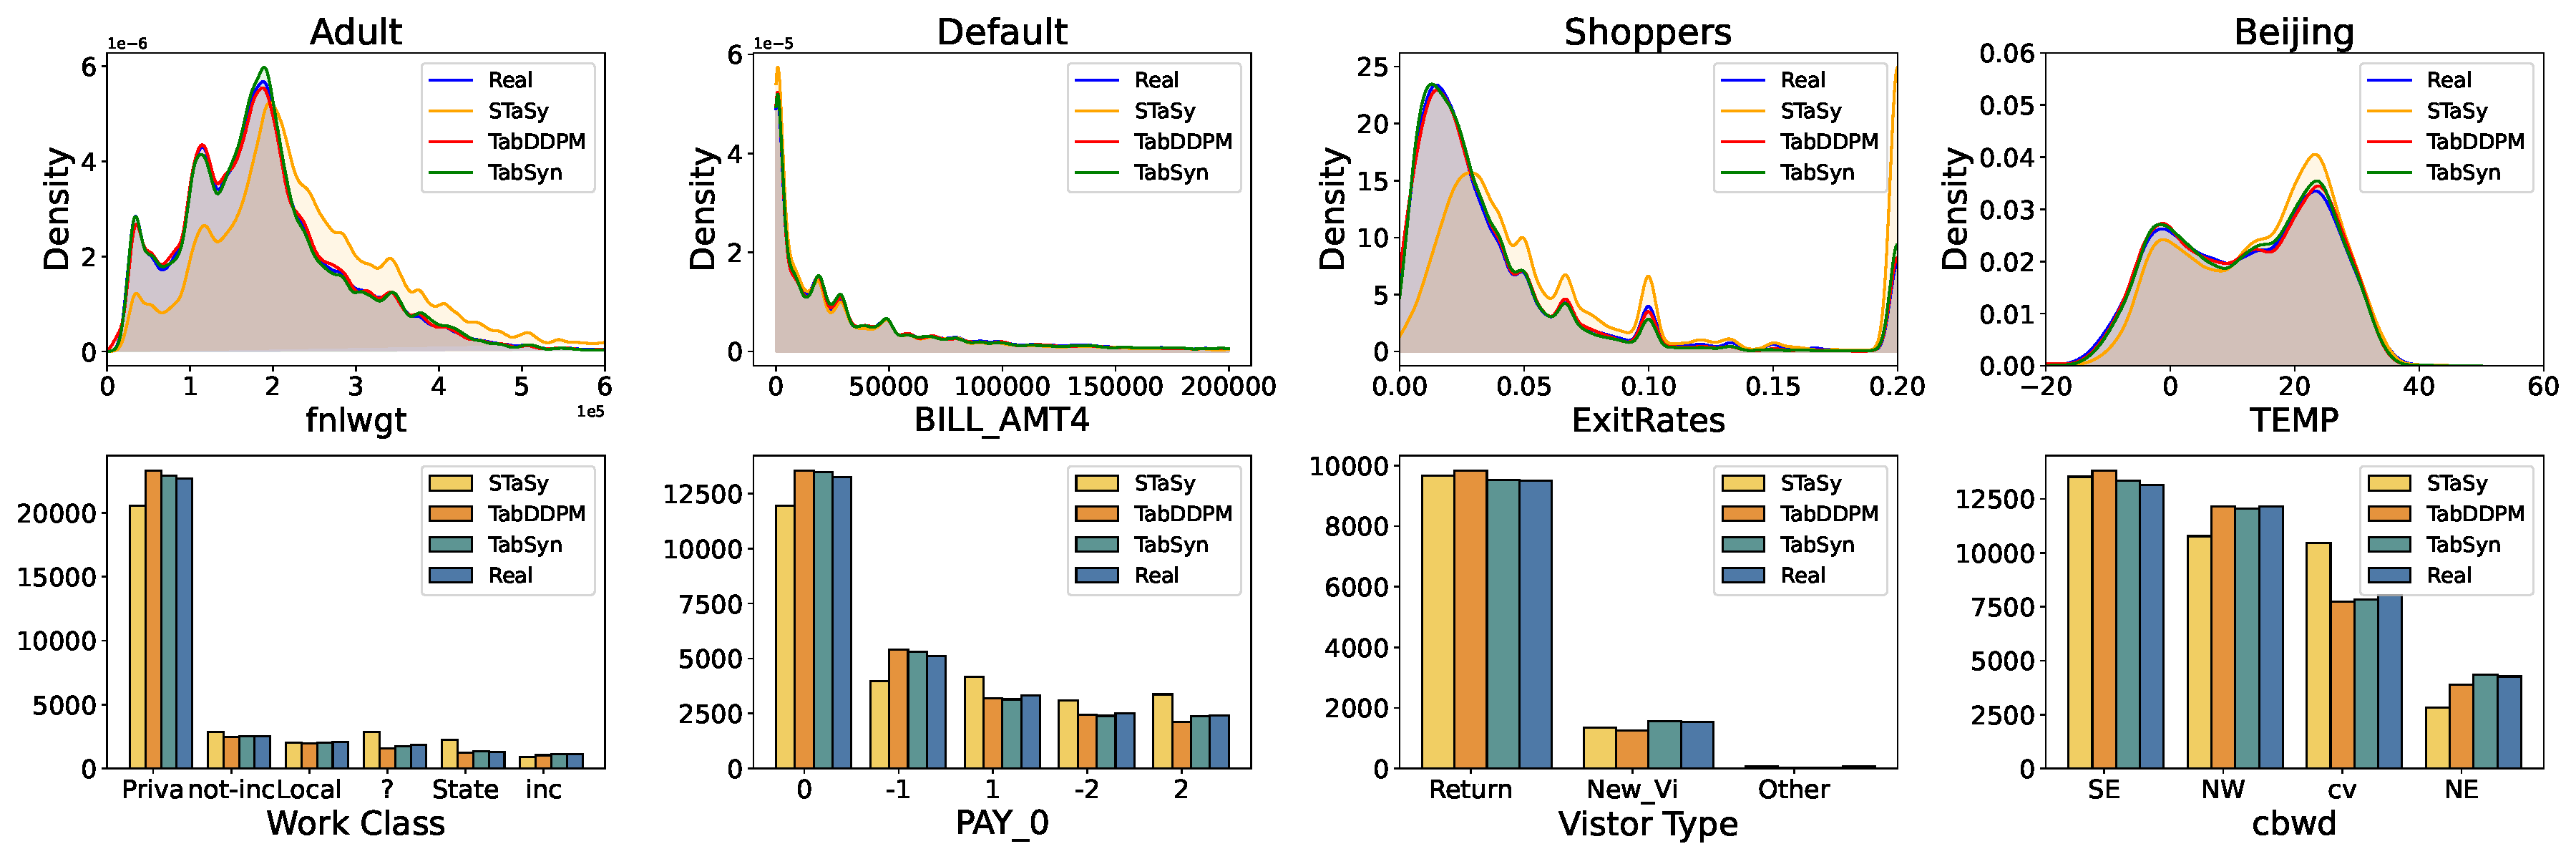
\includegraphics[width = 0.95\linewidth]{Fig/density.pdf}
  \caption{Visualization of synthetic data's single column distribution density (from STaSy, TabDDPM, and \modelname) v.s. the real data. Upper: numerical columns; Lower: Categorical columns. Note that numerical columns show competitive performance with baselines, while \modelname excels in estimating categorical column distributions.}
  \label{fig:case-single}
\end{figure}
\begin{figure}[t]
    \centering
    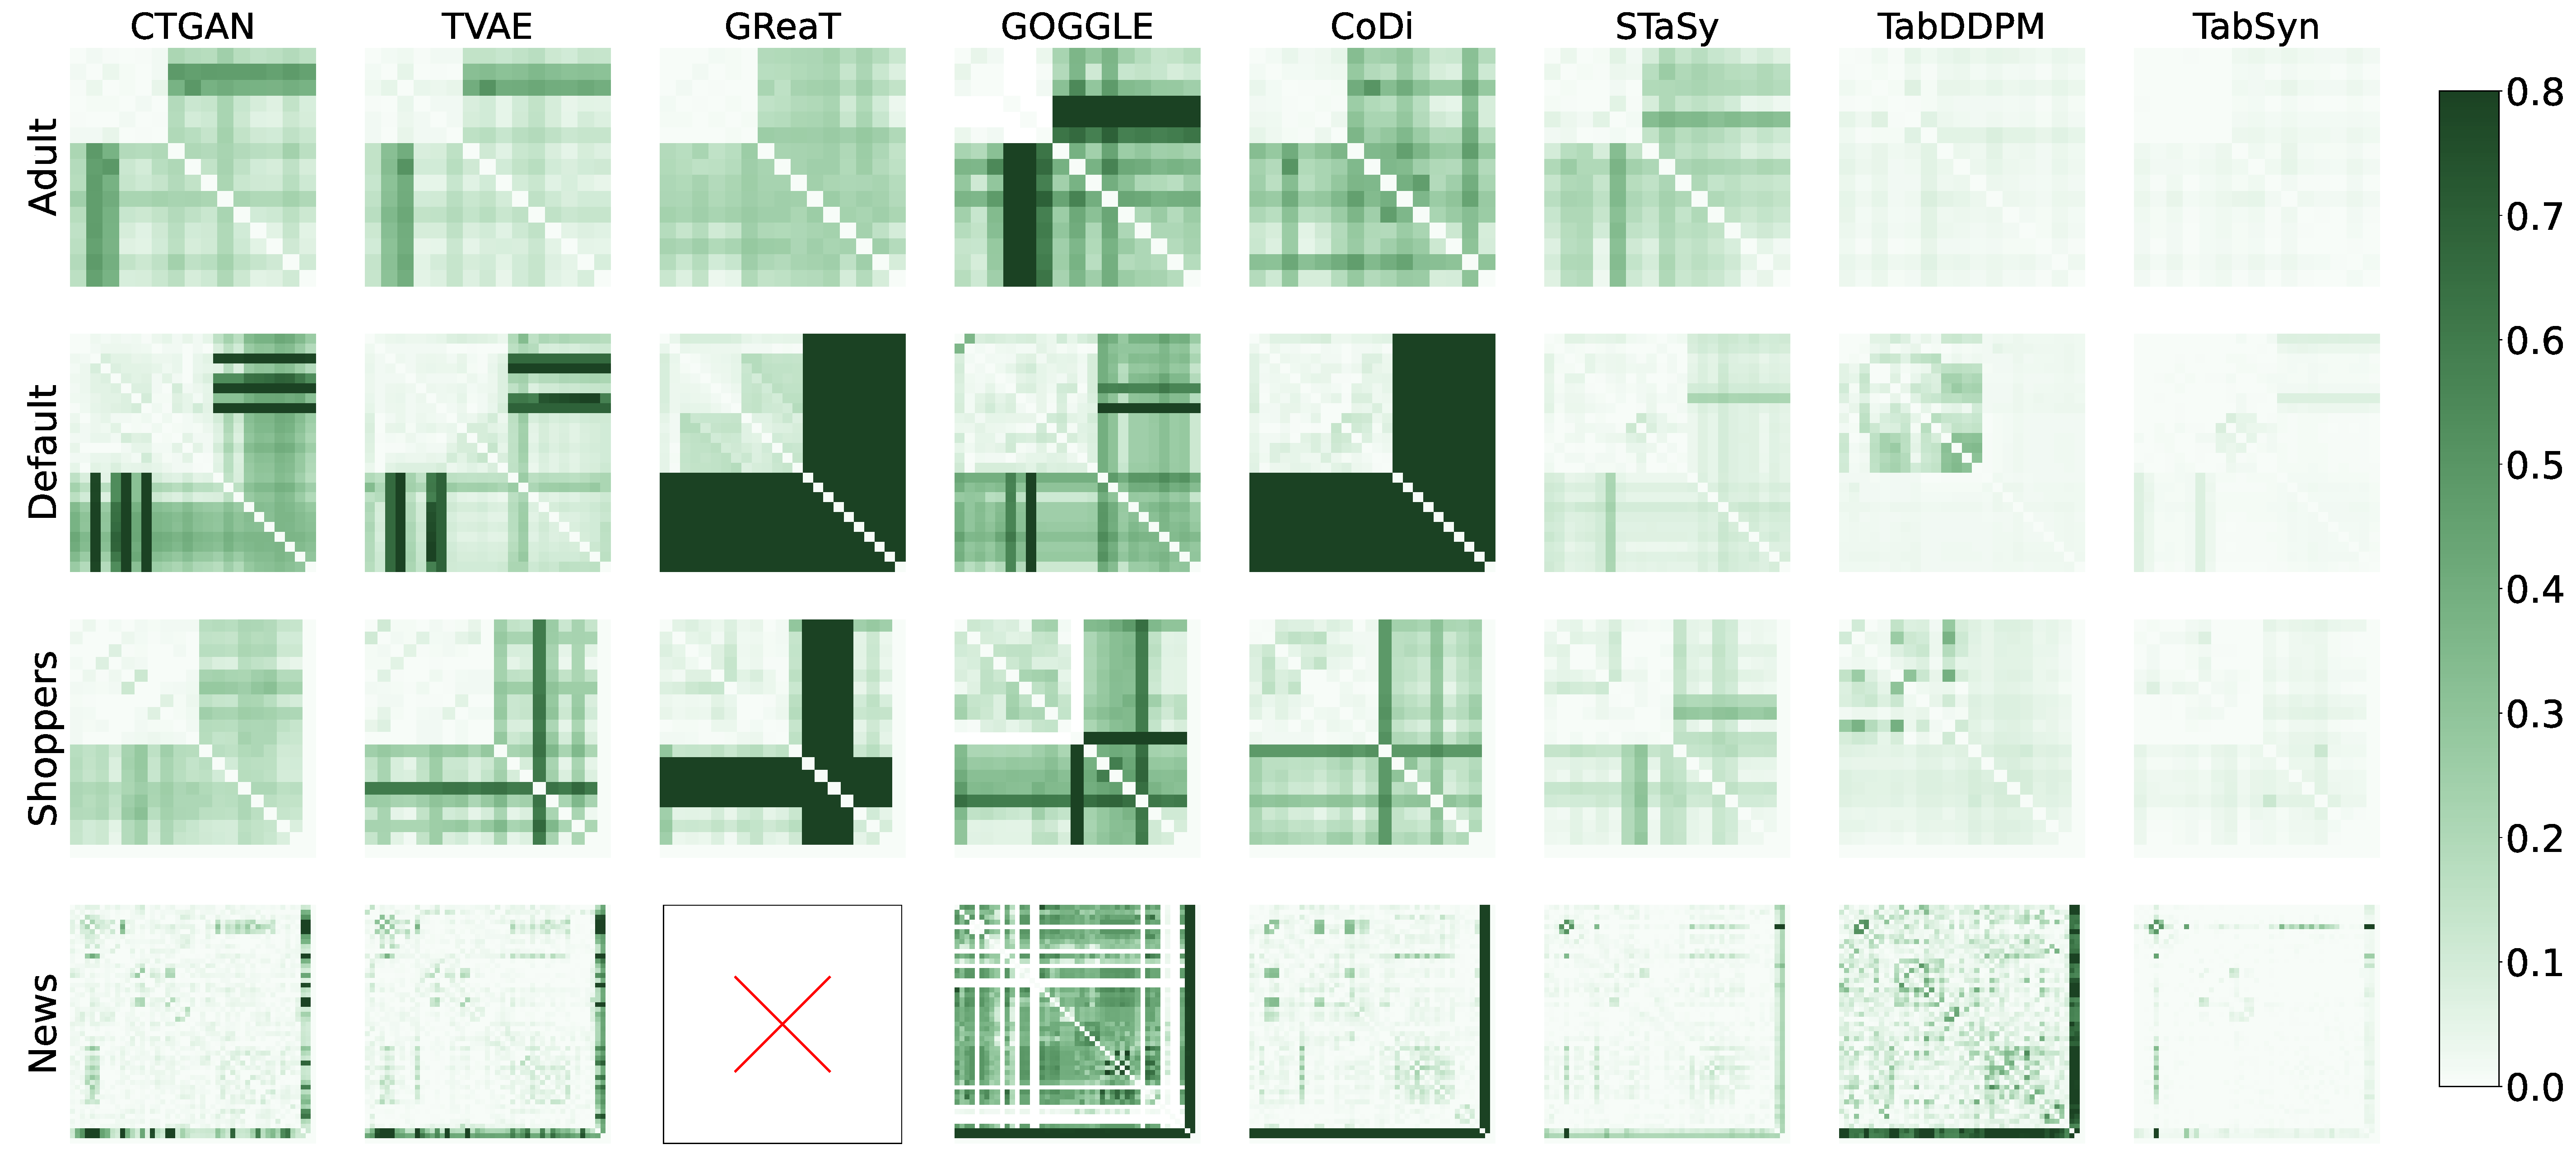
\includegraphics[width = 0.95\linewidth]{Fig/heat_map.pdf}
    \caption{Heatmaps of the pair-wise column correlation of synthetic data v.s. the real data. The value represents the absolute divergence between the real and estimated correlations (the lighter, the better). \modelname gives the most accurate column correlation estimation.}
    \label{fig:case-pair}
    \vspace{-10pt}
\end{figure}

\vspace{-4pt}
